\documentclass{standalone}
\usepackage{tikz}
\usepackage{amsmath}
\usepackage{pgfplots}
\usetikzlibrary{calc,positioning,shapes.misc,shapes.multipart,quotes}
\newcommand{\FixedLengthArrow}{2,0}
\begin{document}
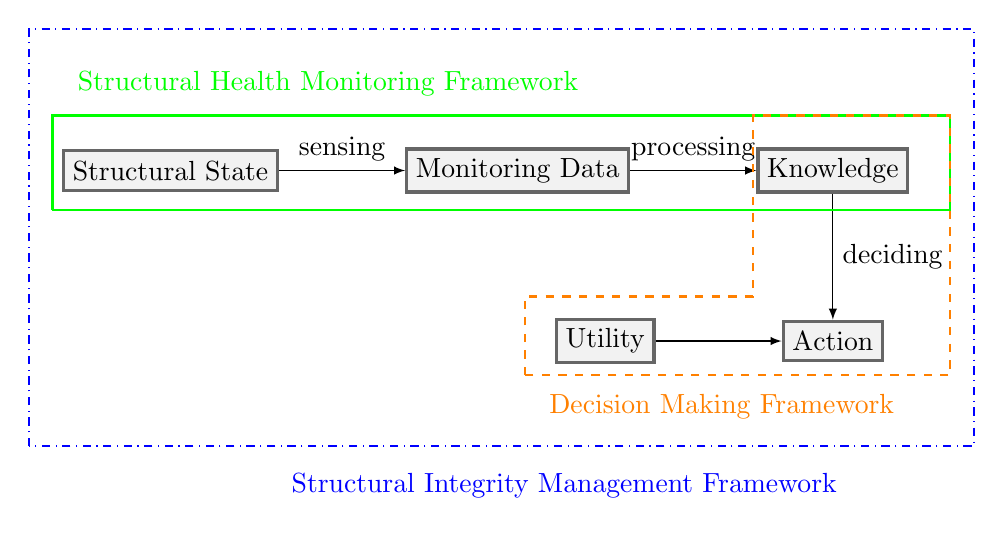
\begin{tikzpicture}[
	roundnode/.style={circle, draw=green!60, fill=green!5, very thick, minimum size=7mm},
	squarednode/.style={rectangle, draw=black!60, fill=black!5, very thick, minimum size=5mm},
	node distance= 1.6cm
	]
	%Nodes
	\node[squarednode](StructuralState){Structural State};
	\node[squarednode](MonitoringData)[right=of StructuralState] {Monitoring Data};
	\node[squarednode](Knowledge)[right=of MonitoringData] {Knowledge};
	\node[squarednode](Action)[below=of Knowledge] {Action};
	\node[squarednode](Utility)[left=of Action] {Utility};
	%Lines
	\draw [-latex](StructuralState) edge["sensing"](MonitoringData);
%	\draw[-latex] (StructuralState.east) --   (MonitoringData.west) node[xshift = -8.2mm,yshift=3mm]{sensing};
	\draw [-latex](MonitoringData) edge["processing"] (Knowledge);
%	\draw[-latex] (MonitoringData.east) -- (Knowledge.west)node[xshift = -8.2mm,yshift=3mm]{processing};
	\draw [-latex](Knowledge) edge["deciding"](Action);
%	\draw[-latex] (Knowledge.south) -- (Action.north)node[xshift = 4.5ex,yshift = 7mm]{deciding};
	\draw[-latex] (Utility.east) -- (Action.west);
	% Draw different schemes
	\draw[green,thick] (-1.5,-0.5) --++ (0,1.2) --++ (11.4,0) --++ (0,-1.2)--(-1.5,-0.5);
	
	\draw[dashed,orange,thick] (4.5,-2.6) --++ (0,1.0) --++ (2.9,0) --++ (0,2.3)--++(2.5,0) --++(0,-3.3) -- (4.5,-2.6);
	
	% Denote the name of the framework

	\draw (2,1.1)node [green]{Structural Health Monitoring Framework};	
	\draw (7,-3)node [orange]{Decision Making Framework};	
	% Draw a unified framework
	\draw[dash dot,blue,thick] (-1.8,-3.5) rectangle (10.2,1.8);
	\draw (5,-4)node [blue]{Structural Integrity Management Framework};
	 
\end{tikzpicture}
\end{document}